\documentclass[a4paper, 12pt, oneside]{scrbook}
\usepackage[a4paper, left=3cm, right=3cm, top=4cm, bottom=5cm]{geometry}

\usepackage{polyglossia}
\setdefaultlanguage{german}
\usepackage{xltxtra}
\usepackage{datetime}

\usepackage{color}
\usepackage[table]{xcolor}
\usepackage{caption}
\captionsetup{width=0.8\textwidth}
\usepackage{chngcntr}
\counterwithout{footnote}{chapter}
\usepackage{wrapfig}

\usepackage{hyperref}
\hypersetup{unicode=true, hidelinks, german}
\usepackage[all]{hypcap}

\author{Nathanael Philipp, Paul Röwer, Assen Tarlov}
\title{Projektbericht}
\subtitle{Methoden für digitale Textkritik und kollaborative Editionsverfahren}
\date{Februar 2015\\\vspace{18em}
\includegraphics{by-sa.png}}

\usepackage[backend=bibtex8,style=numeric,subentry]{biblatex}
\usepackage[babel]{csquotes}
\defbibheading{bibliography}{\chapter{Literaturverzeichnis}}
\bibliography{quellen}

\newcommand{\superscript}[1]{\ensuremath{^{\textrm{#1}}}}
\newcommand{\subscript}[1]{\ensuremath{_{\textrm{#1}}}}
\renewcommand{\th}[0]{\superscript{th}}
\newcommand{\st}[0]{\superscript{st}}
\newcommand{\nd}[0]{\superscript{nd}}
\newcommand{\rd}[0]{\superscript{rd}}

\begin{document}
\maketitle\newpage
\tableofcontents\newpage
\chapter{Einleitung}

Das vorliegende Projekt beschäftigt sich mit dem Thema der digitalen Textkritik und der kollaborativen Editionsverfahren. 
Ziel der digitalen Textkritik ist eine hypothetische Rekonstruktion des ursprüngliches Textes in digitaler Form zu konstruiren. Der vollständige Rekonstruktionen des Textes lässt sich von der Zusammenarbeit der verschiedenen Abschreiber bilden. Jeder Abschreiber bildet eine eigene Edition, die sich von den anderen unterscheiden kann. Die Ursache der Abweichung kann die Freiheit für eine Verbesserung des Textes sein, sowie auch Fehler beim Lesen oder die Unwissenheit über die Sprache, von der den originalen Text stammt.  

In unserem Projekt hadelt sich um einen Manuskript um das 1440 Jahr und drei Editoren. Die erstellte digitale Edition ist in dem EPUB Format, von dem die zwei verschiedene Versionen - mit und ohne Bilder zur Verfügung stammen. 


\chapter{Texteinordnung}
Der Cod. Pal. germ. 324 ist unter den Titeln "Dietrich und seine Gesellen", "Dietrichs Drachenkämpfe", "Dietrichs erste Ausfahrt" und in der Forschung als "Virginal" bekannt. Dieser ist der älteste von drei vollständigen überlieferten Manuskripten (Linhart Scheubels Heldenbuch, Cod. 5478, Dresdner Heldenbuch, Mscr. M 201). Gefertigt wurde der Cod. Pal. germ. 324 um 1440 in der Werkstatt des Diebold Lauber. Die Virginal besitzt 1097 Strophen im Bernerton und 46 kolorierte Federzeichnungen.\cite{ubheidelber_bibpal}

\section{Schrift}
\begin{wrapfigure}{r}{0.5\textwidth}
	\vspace{-40pt}
	\centering
	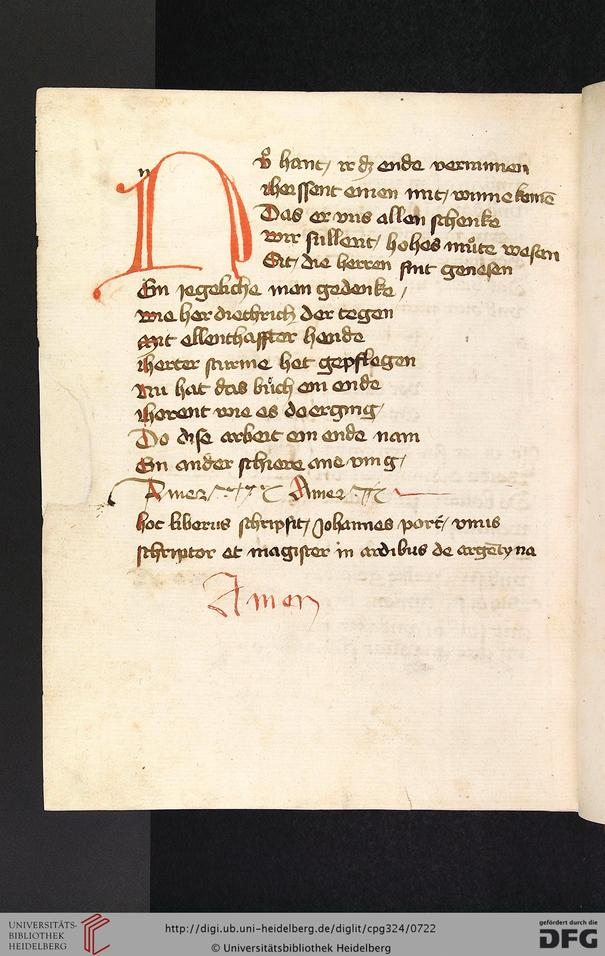
\includegraphics[width=0.4\textwidth]{0722.jpg}
	\caption{Rückseite Blatt 352\cite{virginal352v}}
	\label{fig:1}
\end{wrapfigure}

An der Handschrift waren drei unterschiedliche Schreiber beteiligt. Die folgende Aufteilung wurde dabei vorgenommen: Vom Anfang des Werkes bis zur Vorderseite des Blattes 95 Zeile 6, von dort an bis zu Vorderseite des Blattes 103, wo der letzte Abschnitt beginnt. Die Schreiber sind bis auf den letzten unbekannt, dieser war Johannes Port, ein Straßburger Lohnschreiber. Diese Information entnahm man dem Explicit auf der Rückseite des Blattes 352 im Virginal, hier in Grafik \ref{fig:1} abgebildet.

\begin{wrapfigure}{r}{0.5\textwidth}
	\centering
	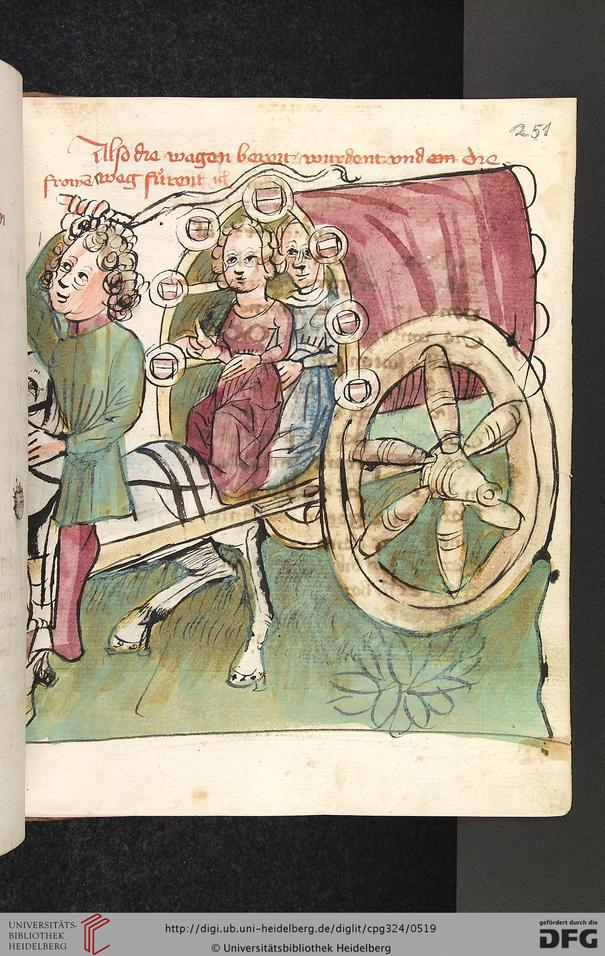
\includegraphics[width=0.4\textwidth]{0519.jpg}
	\caption{Vorderseite Blatt 251\cite{virginal251r}}
	\label{fig:2}
\end{wrapfigure}

Wer die Abschrift in Auftrag gab ist auch ungeklärt, die Illustrationen von mehreren Wappen auf der Vorderseite des Blattes 251 ließen sich nicht eindeutig zuordnen, siehe Grafik \ref*{fig:2}.\cite{ubheidelber_bibpal}
\newpage

\section{Dichtform}
Das ganze Werk ist wie bereits erwähnt im Bernerton verfasst. Entstanden ist diese im 13. Jahrhundert im schwäbisch-alemannischen Raum und wurde nach der Heldenfigur "Dietrich von Bern" benannt. Die mittelalterliche Heldendichtung des Virginals unterliegt so einer festen Strophenform und Melodie. Eine Strophe hat 13 Verse in folgender metrischer Form: 4ma 4ma 3wb 4mc 4mc 3wb 4md 3we 4md 3we 4mf 3wx 3mf. Das bedeutet, "der erste Vers ist ein Vierheber mit männlicher Kadenz (4m), der dritte Vers ist ein Dreiheber mit weiblicher Kadenz (3w) und das Reimschema (der jeweils dritte Buchstabe) ist aab ccb dede fxf."\cite{wiki_bernerton} Als Beispiel dient eine Stelle aus dem Cod. Pal. germ. 324:\\

\begin{tabular}{lr}
Der Berner wart gar schame \textcolor{red}{rot}, & a \\
er leit an sime hertzen \textcolor{red}{not}, & a \\
das jme keine \textcolor{blue}{ofenture} & b \\
By sinen ziten was \textcolor{yellow}{bekant}, & c \\
er gedocht' an meister \textcolor{yellow}{Hiltebrant}: & c \\
"der sol mir geben \textcolor{blue}{sture}." & b \\
Vrlop er zu den frowen \textcolor{green}{nam}, & d \\
er in nicht gesagen \textcolor{pink}{kunde}, & e \\
zu Hiltebrante er do \textcolor{green}{kam}, & d \\
dem er sere clagen \textcolor{pink}{begunde}: & e \\
"die frowen hant gefraget \textcolor{orange}{sere} & f \\
mich noch dingen, der ich nicht weis; & x \\
das lit mir an dem hertzen \textcolor{orange}{swere}." & f \\
\end{tabular}\cite{ubh_bernerton}\\

Der Berner war rot vor Scham, er litt Herzensnot. Das keine (Frau) bei ihm sitze war offenbar bekannt. Er wandte sich an Meister Hildebrant: "Der soll mir eine Hure geben!" Er nahm sich frei um zu den Frauen zu gehen. In nicht genannter Kunde ging er dann zu Hildebrant, dem er seine Klagen bekundete: "Die Frauen haben mich sehr nach Dingen gefragt, die ich nicht weiß. Das litt mir schwer am Herzen."\cite{wiki_bernerton}

\section{Illustrationen}
Die Federzeichnungen sind in der Werkstatt Diebold Laubers von Zeichnergruppen gefertigt worden. Sie spiegeln das höfische Leben mit seinen Sitten und Gebräuchen wieder. Es werden Kampf-, Dialog- sowie Abreiseszenen dargestellt.\cite{ubheidelber_bibpal}

\section{Inhaltliche Einordnung}
Die Virtigal gehört zu Dietrichepik, in der Heldenepik zieht der junge Dietrich von Bern mit seinem Waffenmeister Hildebrand zu Abenteuern aus. 

"Im Heidelberger Virginal (Cpg 324; Papierhandschrift, um 1440, 1097 Strophen) ziehen Hildebrand und Dietrich ins Waldgebirge von Tirol, um gegen den Heiden Orkise zu kämpfen, der in das Land der Königin Virginal eingefallen ist. Hildebrand findet ein Mädchen aus Virginals Gefolge, das zum Tribut für Orkise bestimmt ist. Er besiegt Orkise. Dietrich ist inzwischen in Kampf mit einer ganzen Schar von Heiden verwickelt. Hildebrand hilft ihm, sie zu besiegen. Das Mädchen lädt die beiden nach Königin Virginals Residenz Jeraspunt ein. Sie geht voraus, Virginal schickt ihnen den Zwerg Bibung entgegen. Dietrich und Hildebrand sind aber in einen Kampf gegen Drachen geraten. Einer davon hat einen Ritter im Maul. Hildebrand kann den Drachen töten, der Ritter ist Rentwin, Sohn des Helferich und ein Großneffe Hildebrands. Hildebrand und Dietrich gehen nach Arona, der Residenz von Rentwins Eltern Helferich. Dort findet sie Bibung und überbringt Virginals Einladung. 14 Tage später brechen Hildebrand und Dietrich mit Helferich und Gefolge auf. Dietrich reitet voraus, verirrt sich, gelangt zur Burg Muter. Der Riese Wicram, mit anderen Riesen im Dienste von Nitger, dem Burgherrn von Muter, überwältigt ihn und bringt ihn zu Nitger, der ihn gefangen setzt. Doch kümmert sich Nitgers Schwester Ibelin um Dietrich. Sie sendet eine Nachricht nach Jeraspunt. Daraufhin holt man Dietrichs Gefolgsleute aus Bern, den König Iman von Ungarn und Biterolf und Dietleib zu Hilfe. Nach Sammlung in Jeraspunt ziehen sie nach Muter. In elf Zweikämpfen werden alle Riesen erschlagen. Nitger muss sein Land von Dietrich zu Lehen nehmen. Auf dem Weg nach Jeraspunt kommt es wieder zu elf Einzelkämpfen mit Riesen und wieder zu Drachenkämpfen. Angekommen gibt es ein großes Fest. Auf eine Nachricht von einer drohenden Belagerung Berns hin kehren Dietrich und seine Gesellen nach Hause zurück."\cite{wiki_virginal}

\chapter{Projektarbeit}
Im folgenden werden wir zunächst auf den Ablaufplan eingehen, den wir zu beginn aufgestellt haben. Im Anschluss daran werden wir unsere Erfahrungen bei der Transkription erläutern. Des weiteren beschreiben wir kurz die benutzen Tools und abschließend das fertige Produkt.

\section{Ablaufplan}
Wir haben uns zunächst einen Ablaufplan überlegt und die uns zur Verfügung stehende Zeit in drei Phasen eingeteilt. In der ersten Phase haben wir uns mit der Transkription selbst beschäftigt und haben die ersten 10 Seiten abgeschrieben. Wir haben dabei die Abschrift von Friedrich Heinrich von der Hagen\cite{fhvdh_helden} als Hilfestellung benutzt.

In der zweiten Phase haben wir als erstes aus unseren drei einzelnen Abschrift zusammengeführt und diese ins EpiDoc-Format gebracht. Anschließen haben wir daraus ein EPUB erstellt. Des weiteren haben wir unsere Abschrift mit der von Friedrich Heinrich von der Hagen vergleichen und einen kritischen Apparat erstellt.

In der dritten und letzten Phase haben wir das EPUB fertig gestellt und diesen Bericht geschrieben.
\section{Transkription}
\subsection{Nathanael Philipp}
Nach ersten Schwierigkeiten den Text zu lesen und zu entziffern habe ich nach einem nebeneinanderlegen der Handschrift und der Abschrift von Friedrich Heinrich von der Hagen sehr schnell in den Text gefunden und war in der Lage ohne allzu große Schwierigkeiten die Handschrift abzuschreiben. Allerdings habe ich anstelle der F's in der Abschrift von von Hagen S's gelesen, ebenso hat von Hagen viele Bögen über den Buchstaben gesehen.

\subsection{Paul Röwer}
Das Transkriptionsprojekt hat mir als Informatiker gezeigt, wie umfangreich die Aufarbeitung alter Textüberliefungen ist. Durch diese kann man viel historisch relevantes Wissen ziehen, wie über den geschichtlichen Verlauf der Welt oder auch literarische Ausdrucksformen. Des Weiteren ist es wichtig bereits gegenwärtige oder neue Technologien  zu-oder weiterzuentwickeln um die Arbeit in diesem Bereich zu unterstützen. Beispielsweise ist das "Optical Character Recognition" weiter auf Handschriften zu trainieren oder eine Verfahren, welches bei der Erstellung von Prosaformen aus alten Dichtungen generiert, zu erfinden.

\subsection{Assen Tarlov}

Die Transkriptionarbeit war am Anfang schwierig, weil man nicht mit der Schrift gewöhnt ist. Die erste Zeile habe ich mit Hilfe der Abschrift von Friedrich Heinrich transkibiert, was mir geholfen hat, sich an die Schrift zu orientieren. Die Frage ist, ob es möglich wäre ein "OCR" zu entwickeln, die den Text automatisch transkribiert. Die Aufgabe wäre nicht leicht, da der Text nicht die perfekte Qualität hat und die Machine muss ein explizites Wissen über die Sprache in dieser Periode lernen.

\section{Tools und Formate}
Die einzelnen Abschriften haben wir im EpiDoc-Format zusammengeführt. Dabei handelt es sich um ein XML-Format das ein strukturiertes Markup von epigraphischen Dokumenten in TEI-XML definiert.

Da EPUB mit den XML Dateien vom EpiDoc nicht direkt arbeiten kann haben wir ein kleines Pythonskript geschrieben das aus dem XML einfaches HTML macht. Anschließend haben wir mit Hilfe von Calibre aus den HTML-Dateien das EPUB erstellt.

Bei Calibre\cite{calibre} handelt es sich um ein Medienverwaltungssystem, das vorallem auf EBooks ausgelegt ist und Tools für deren Erstellung/Bearbeitung mitbringt.

Mit Juxta\cite{juxta} haben wir den kritischen Apparat zwischen unserer Abschrift und der von  Friedrich Heinrich von der Hagen erstellt, diese ist ebenfalls im EPUB enthalten.

\newpage
\section{Produkt}
Wir haben uns entschieden zwei verschiedene EPUB Versionen zu erstellen. In der ersten ist neben unserer Abschrift zu jedem Absatz unserer Abschrift das Digitalisat mit eingebunden. Durch die vielen Bilder ist diese Version allerdings sehr groß geworden und wir haben deshalb die zweite Version erstellt, die die Digitalisate nicht enthält.

Im EPUB sind die ersten drei Kapitel enthalten und entsprechend in Absätze gegliedert. Nach der Abschrift ist der kritischer Apparat enthalten.

Wir wollten zuerst die Digitalisate neben der Abschrift anzeigen, allerdings ist dies nicht für mobile Endgeräte geeignet, deswegen haben wir uns dafür entschieden sie nacheinander anzuzeigen, aber es sind Verknüpfungen enthalten. Man könnte sich überlegen eine extra Version für die mobilen Endgeräte entwerfen.

\chapter{Fazit}

Dieses Projekt hat uns gezeigt, wie schwierig und umfangreich textkritik-und editieren seien können. Das Projekt haben wir in drei Phasen eingeteilt und zu der jeden Phase waren wir mit verschiedenen Problemen begegnet. 

Das Problem bei der ersten Phase war hauptsächlich das Lesen von dem Text. Diese Fehler kann man in dem kritischen Apparat gesehen werden - ein typischer Fehler ist "s" mit "f" und umgekehrt zu verwächseln, sowie "u" mit "v". Die Abschrift von Friedrich Heinrich war ein hilfreiches Mittel sich an die originale Schrift zu orientieren und die Fehler zu minimieren.

Die zweite Phase ist das Erstellen von dem EpiDoc und anschließend EPUB. Das EpiDoc Format ist nicht mit dem EPUB kompatibel und ein Python-Script war nötig, um das Problem zu beheben. 

Bei der dritten Phase handelt sich um das Erstellen von den fertigen EPUB-Versionen mit Hilfe des Calibre-Programs. Der Text haben wir zentriert. Bilder von der Manuscript haben wir mit dem GIMP-Programm zu jedem Absatz geordnet und eingefügt. Die Zeile des Absatzes waren nicht immer auf einer Seite, was eine Einordnung der Bilder nötigte. 

Probleme, die in der Zukunft noch zu beheben könnten, sind Named-Entities. Named-Entities sind solche Elemente in dem Text, die klassifierzt werden können - z.B Namen von Personen, Organisationen, Orten. Diese Namen können extrahiert und in einer Liste gespeichert werden. Anhand von dieser Liste können Fehler, aufgrund von falsch geschriebenen Namen korrigiert werden. 


Was kann man mit der Edition noch machen ? 

Eine Möglichkeit wäre die Abschrift ins Hochdeutsche zu übersetzen. Das Übersetzen wird der Text verständlicher und zu mehreren Leute attraktiver machen. 
Querverweise können z.B. automatisch gefunden und eingefügt werden. Eine morphologische Syntax oder finden von alten Wörtern bzw. die Entwicklung der Bedeutung mit der Zeit wären andere Ideen mit den man sich mit dieser Edition beschäftigen kann. 
 

\printbibliography
\end{document}